%iffalse           
\let\negmedspace\undefined
\let\negthickspace\undefined
\documentclass[journal,12pt,onecolumn]{IEEEtran}
\usepackage{cite}
\usepackage{amsmath,amssymb,amsfonts,amsthm}
\usepackage{algorithmic}
\usepackage{graphicx}
\usepackage{textcomp}
\usepackage{xcolor}
\usepackage{txfonts}
\usepackage{listings}
\usepackage{enumitem}
\usepackage{mathtools}
\usepackage{gensymb}
\usepackage{comment}
\usepackage[breaklinks=true]{hyperref}
\usepackage{tkz-euclide} 
\usepackage{listings}
\usepackage{gvv}                                        
\def\inputGnumericTable{}                                 
\usepackage[latin1]{inputenc}                                
\usepackage{color}                                            
\usepackage{array}                                            
\usepackage{longtable}                                       
\usepackage{calc}                                             
\usepackage{multirow}                                         
\usepackage{hhline}                                           
\usepackage{ifthen}                                           
\usepackage{lscape}

\newtheorem{theorem}{Theorem}[section]
\newtheorem{problem}{Problem}
\newtheorem{proposition}{Proposition}[section]
\newtheorem{lemma}{Lemma}[section]
\newtheorem{corollary}[theorem]{Corollary}
\newtheorem{example}{Example}[section]
\newtheorem{definition}[problem]{Definition}
\newcommand{\BEQA}{\begin{eqnarray}}
\newcommand{\EEQA}{\end{eqnarray}}
\newcommand{\define}{\stackrel{\triangle}{=}}
\theoremstyle{remark}
\newtheorem{rem}{Remark}
\usepackage{circuitikz}
\begin{document}

\bibliographystyle{IEEEtran}
\vspace{3cm}
\title{Assignment-2}
\author{AI24BTECH11027- R Sumanth % <-this % stops a space
}
\maketitle
\bigskip

\textbf{\section{Vector Arithmetic(CBSE)}}

\textbf{Question:} $\vec{\brak{-1,2,1}}$, $\vec{\brak{1,-2,5}}$, $\vec{\brak{4,-7,8)}}$ and $\vec{\brak{2,-3,4}}$ are the vertices of a parallelogram.
\begin{table}[h!]
\renewcommand{\thetable}{1}
    \centering
   \begin{tabular}{|c| c |  c |}
\hline
\textbf{Variable} & \textbf{Value} & \textbf{Description} \\
\hline
$A$ & \myvec{-1 \\ 2\\ 1\\ \\} & $A$ defined as point \\
\hline
$B$ & \myvec{1 \\ -2\\ 5\\}  & $B$ defined as point  \\
\hline
$C$ & \myvec{4 \\ -7\\ 8\\} & $C$ defined as point\\
\hline
$D$ & \myvec{2 \\ -3\\ 4\\} & $D$ defined as point \\
\hline
\end{tabular} 
   \def\tablename{Table}
   \caption{Variables Used}
\end{table}

\solution property : opposite sides of parallelogram are equal.\\ 

$\Vec{A}(-1, 2, 1), \vec{B}(1, -2, 5), \vec{C}(4, -7, 8), \vec{D}(2, -3, 4)$ 

\begin{align}
AB&=B-A =\myvec{1 - (-1)\\ -2 - 2\\ 5 - 1} =\myvec{2\\ -4\\ 4}\\ 
BC&=C-B =\myvec{4 - 1\\ -7 - (-2)\\ 8 - 5} =\myvec{3\\ -5\\ 3}\\ 
CD&=D-C =\myvec{2 - 4\\ -3 - (-7)\\ 4 - 8} = \myvec{-2\\ 4\\ -4}\\ 
DA&=A-D =\myvec{-1 - 2\\ 2 - (-3)\\ 1 - 4} = \myvec{-3\\ 5\\ -3}  
\end{align}

Verify if $AB$ is equal to $ CD $ and $ BC $ is equal to $ DA $:
\begin{align}
AB+CD&=\myvec{2\\ -4\\ 4}+\myvec{-2\\ 4\\ -4}=\myvec{0\\ 0\\ 0}\\
BC+DA&=\myvec{3\\ -5\\ 3}+\myvec{-3\\ 5\\ -3}=\myvec{0\\ 0\\ 0}
\end{align}

Since $AB + CD = 0 $ and $ BC+ DA = 0 $, the quadrilateral formed by the points is a parallelogram.

\begin{figure}[h!]
   \centering
   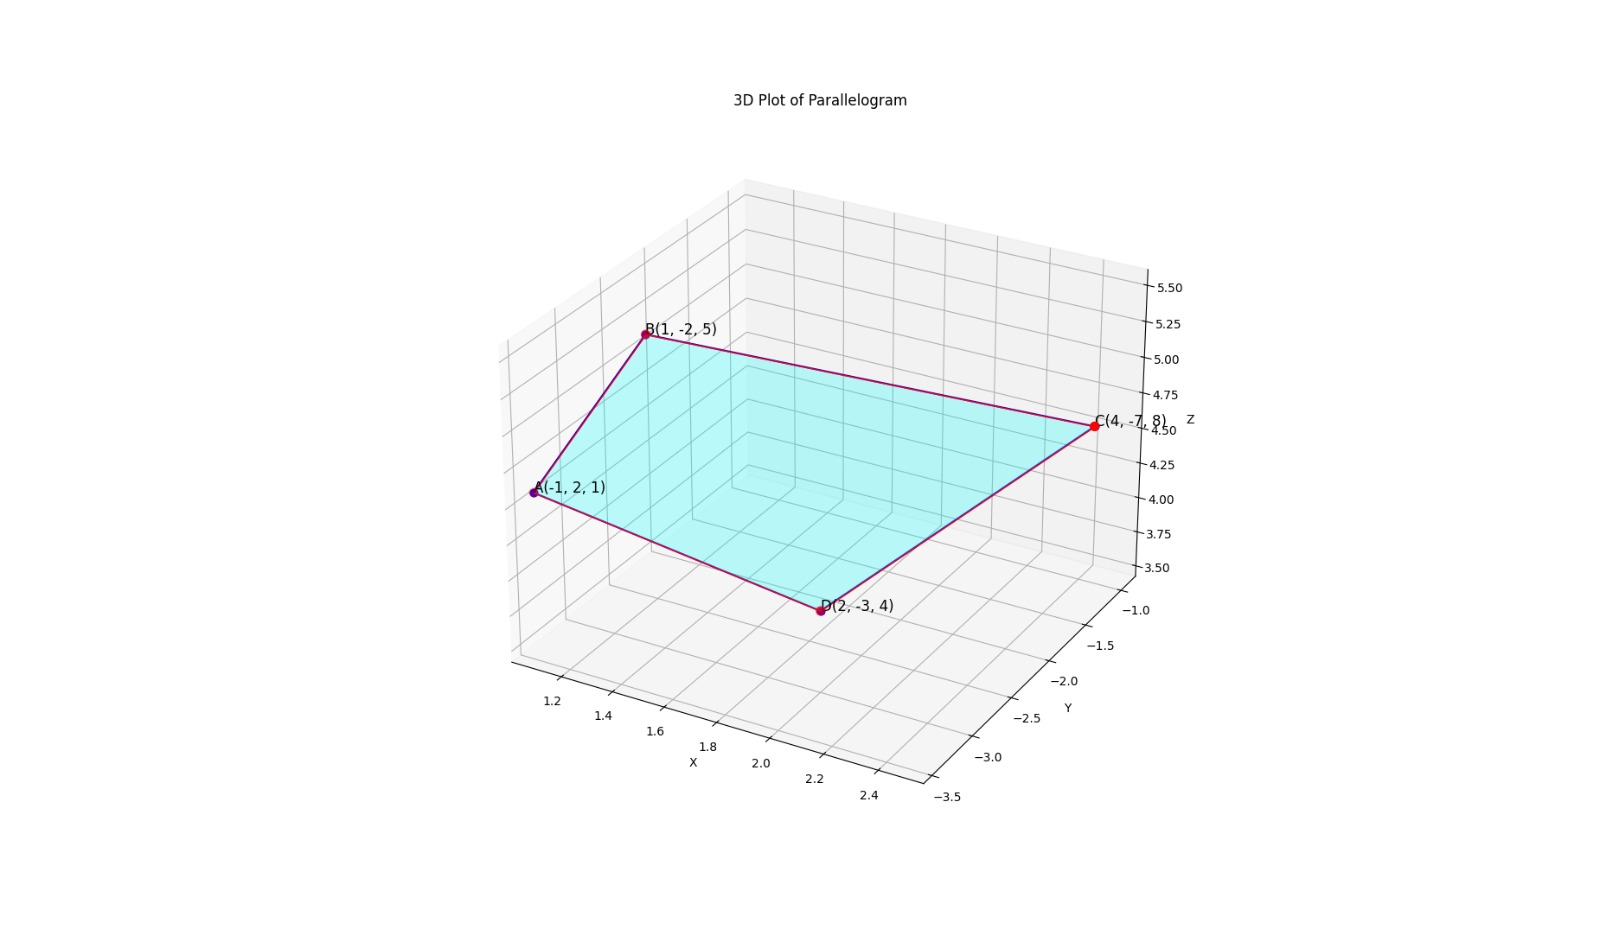
\includegraphics[width=1.1\linewidth]{IMG.jpg}
   \caption{Stem Plot of y\brak{n}}
     \label{stemplot}
\end{figure}
\end{document}  
